% Author: Joseph Rowell
% Version: 3.0
% This work is licensed under a Creative Commons Attribution 4.0 International License.
\documentclass[12pt, a4paper]{report}
\usepackage[a4paper, total={6.25in, 8.25in}]{geometry} %%%%%% CHECK MARGIN REQ. 8.25 in?
% References
\usepackage{natbib}
\setcitestyle{authoryear,open={(},close={)}}

\usepackage{multirow}
%\usepackage{multicol}
\usepackage{array}

\usepackage[T1]{fontenc}
\usepackage[utf8]{inputenc}
\usepackage[english]{babel}
\usepackage{siunitx}
\usepackage{graphicx}
\usepackage{tipa} % for the \ark{} command
\usepackage{graphics} % for pdf, bitmapped graphics files
%\usepackage{times} % assumes new font selection scheme installed
\usepackage{amsmath}
\usepackage{latexsym}
\usepackage{amscd}% for commutative diagrams
\usepackage{mathrsfs} %this package is for the script font \mathscr
\usepackage{relsize}
\usepackage{delarray}

\usepackage{graphicx} % for youtube image link

\usepackage{datatool}% Sorted list http://ctan.org/pkg/datatool

\usepackage{xcolor} % highlight text 
\usepackage[nottoc]{tocbibind} % Adds bibliography to TOC
%Also adds roman numeral pages to TOC

\usepackage{glossaries}

\usepackage{pstricks}
\usepackage{theorem}
\usepackage{changepage}
\usepackage{euscript}
\usepackage{textcomp}
\usepackage{esvect}
\usepackage{parskip}
\usepackage{placeins}
\usepackage{subfigure}
%\usepackage{subcaption}
\usepackage{array}
\usepackage{delarray}
\usepackage{stmaryrd}
\usepackage{fancyhdr}
\usepackage{graphpap}
\usepackage{makeidx}
\usepackage{enumerate}
\usepackage{esint}
\usepackage{datetime}
\usepackage{caption}
\usepackage{smartdiagram}
\usesmartdiagramlibrary{additions}
%Set Abstract Page
\usepackage{abstract}
\setlength{\absleftindent}{-5mm}
\setlength{\absrightindent}{-5mm}

%Colour definitions - put before TikZ
\usepackage{color}
\definecolor{igreen}{rgb}{0.0, 0.56, 0.0}
\usepackage{xcolor, colortbl}
\colorlet{gred}{-red!75!green!65!}
\colorlet{mamber}{-red!75!green!15!blue!50!}
\colorlet{grown}{-red!75!blue!20!green}
\colorlet{bled}{-red!85!blue!40!green!45!}
\colorlet{waters}{cyan!25} % Define color for the water
\colorlet{water}{cyan!25!green!20!} % Define color for the water
\definecolor{grin}{HTML}{00F9DE}
\usepackage{rotating}
\providecommand{\keywords}[1]{\textbf{\textit{Keywords---}} #1}

% For faint dotted table line
\usepackage{arydshln}
\setlength{\dashlinedash}{.4pt}
\setlength{\dashlinegap}{.8pt}

\usepackage{booktabs}
\usepackage{graphicx}
\usepackage{tikz}

% Added by me
\def\checkmark{\tikz\fill[scale=0.5](0,.35) -- (.25,0) -- (1,.7) -- (.25,.15) -- cycle;}

\usepackage{tikz-3dplot}
\usetikzlibrary{
arrows,
arrows.meta,
automata,
backgrounds,
calc,
decorations,
decorations.pathmorphing,
decorations.pathreplacing,
decorations.fractals,
external,
fit,
matrix,
petri,
positioning,
shadows,
shapes,
shapes.multipart,
topaths,
intersections
}
\usepackage{eso-pic}
\def\ba{\begin{array}}
\def\ea{\end{array}}
\def\beann{\begin{eqnarray*}}
\def\eeann{\end{eqnarray*}}
\def\bea{\begin{eqnarray}}
\def\eea{\end{eqnarray}}
\def\bsy{\boldsymbol}
\def\gray#1{{\color{gray}#1}}

%% COUNTERS
\setcounter{MaxMatrixCols}{20}
\renewcommand{\thesection}{\arabic{section}}
\renewcommand{\thesection}{\thechapter.\number\numexpr\value{section}}
\renewcommand{\thesubsection}{\thesection.\number\numexpr\value{subsection}}
%%For changemargin
\def\quote{\list{}{\rightmargin\leftmargin}\item[]}
\let\endquote=\endlist 
\def\changemargin#1#2{\list{}{\rightmargin#2\leftmargin#1}\item[]}
\let\endchangemargin=\endlist 
\makeatletter
\newlength\qvec@height
\newlength\qvec@depth
\newlength\qvec@width
\newcommand{\qvec}[2][]{
    \settoheight{\qvec@height}{$#2$}
    \settodepth{\qvec@depth}{$#2$}
    \settowidth{\qvec@width}{$#2$}
  \def\qvec@arg{#1}
  \raisebox{.2ex}{\raisebox{\qvec@height}{\rlap{% 
    \kern.05em
    \begin{tikzpicture}[scale=1,shorten >=-3pt,shorten <=-3pt]
    \pgfsetroundcap
    \coordinate (Stx) at (.05em,0) ;
		\coordinate (Arx) at (\qvec@width-.05em,0) ;
    \draw[->](Stx) to[bend left] (Arx);
    \end{tikzpicture}
  }}}
  #2
}
\makeatother
\makeatletter
\newlength\pvec@height
\newlength\pvec@depth
\newlength\pvec@width
\newcommand{\pvec}[2][]{
    \settoheight{\pvec@height}{$#2$}
    \settodepth{\pvec@depth}{$#2$}
    \settowidth{\pvec@width}{$#2$}
  \def\pvec@arg{#1}
  \raisebox{.2ex}{\raisebox{\pvec@height}{\rlap{% 
    \kern.05em
    \begin{tikzpicture}[scale=1,shorten >=-3pt,shorten <=-3pt]
    \pgfsetroundcap
    \coordinate (Stx) at (.05em,0) ;
		\coordinate (Arx) at (\pvec@width-.05em,0) ;
    \draw[->](Stx) to[bend right] (Arx);
    \end{tikzpicture}
  }}}
  #2
}
\makeatother
\makeatletter
\newlength\vvec@height%
\newlength\vvec@depth%
\newlength\vvec@width%
\newcommand{\vvec}[2][]{%
  \ifmmode%
    \settoheight{\vvec@height}{$#2$}%
    \settodepth{\vvec@depth}{$#2$}%
    \settowidth{\vvec@width}{$#2$}%
  \else 
    \settoheight{\vvec@height}{#2}%
    \settodepth{\vvec@depth}{#2}%
    \settowidth{\vvec@width}{#2}%
  \fi%
  \def\vvec@arg{#1}%
  \def\vvec@dd{:}%
  \def\vvec@d{.}%
  \raisebox{.2ex}{\raisebox{\vvec@height}{\rlap{%
    \kern.05em%
    \begin{tikzpicture}[scale=1]
    \pgfsetroundcap
    \draw (.05em,0)--(\vvec@width-.05em,0);
    \draw (\vvec@width-.05em,0)--(\vvec@width-.15em, .075em);
    \draw (\vvec@width-.05em,0)--(\vvec@width-.15em,-.075em);
    \ifx\vvec@arg\vvec@d%
      \fill(\vvec@width*.45,.5ex) circle (.5pt);%
    \else\ifx\vvec@arg\vvec@dd%
      \fill(\vvec@width*.30,.5ex) circle (.5pt);%
      \fill(\vvec@width*.65,.5ex) circle (.5pt);%
    \fi\fi%
    \end{tikzpicture}%
  }}}%
  #2%
}
\makeatother
\def\ba{\begin{array}}
\def\ea{\end{array}}
\def\beann{\begin{eqnarray*}}
\def\eeann{\end{eqnarray*}}
\def\bea{\begin{eqnarray}}
\def\eea{\end{eqnarray}}
\def\bsy{\boldsymbol}
\def\gray#1{{\color{gray}#1}}
\usepackage{titlesec}
\usepackage{multirow}
%To reference within text
\usepackage{hyperref}
%\usepackage{ieeetr}
\usepackage{lipsum}
\usepackage{tikz-cd}
\usepackage{float}
\usepackage{titling}
\usepackage{epigraph}
\usepackage[title, titletoc]{appendix}
\setlength\epigraphwidth{8cm}
\setlength\epigraphrule{0pt}

\titleformat{\chapter}{\normalfont\LARGE}{\thechapter\,$\vert$}{20pt}{\LARGE}{\setcounter{chapter}{0}}
\setlength{\headheight}{15pt}
\titlespacing*{\chapter}{0pt}{-70pt}{40pt} %Move chapter titles up
% Title page logos:
\makeatletter
\newcommand\BackgroundPicturea[3]{
	\setlength{\unitlength}{1pt}
	\put(0,\strip@pt\paperheight){
		\parbox[t]{\paperwidth}{
			\vspace{#2}\hspace{#3}
			\mbox{\includegraphics[scale=0.5]{#1}}
}}}
\newcommand\BackgroundPictureb[3]{
	\setlength{\unitlength}{1pt}
	\put(0,\strip@pt\paperheight){
		\parbox[t]{\paperwidth}{
			\vspace{#2}\hspace{#3}
			\mbox{\includegraphics[scale=0.3]{#1}}
}}}
\makeatother
% For my abbreviations
\newcommand{\abbrlabel}[1]{\makebox[3cm][l]{\textbf{#1}\ \dotfill}}
\newenvironment{abbreviations}{\begin{list}{}{\renewcommand{\makelabel}{\abbrlabel}}}{\end{list}}
% Line Spacing%%%%%%%%%%%%%%%%%%%%%%%%%%%%%%%%%
\usepackage{setspace}
\setstretch{1.5}
%Set of command is for the changemargin environment
\def\quote{\list{}{\rightmargin\leftmargin}\item[]}
\let\endquote=\endlist 
\def\changemargin#1#2{\list{}{\rightmargin#2\leftmargin#1}\item[]}
\let\endchangemargin=\endlist
%Replace Contents to Table of Contents	
\addto\captionsenglish{
	\renewcommand{\contentsname}%
	{Table of Contents}
	\setcounter{tocdepth}{3}% Include \subsubsection in ToC
	\setcounter{secnumdepth}{3}% Number \subsubsection in ToC
	}
\renewcommand{\listfigurename}{List of Figures}
\renewcommand{\listtablename}{List of Tables}


\usepackage{xcolor}
\usepackage{listings}
\usepackage{xcolor}

%New colors defined below
\definecolor{codegreen}{rgb}{0,0.6,0}
\definecolor{codegray}{rgb}{0.5,0.5,0.5}
\definecolor{codepurple}{rgb}{0.58,0,0.82}
\definecolor{backcolour}{rgb}{0.95,0.95,0.92}

%Code listing style named "mystyle"
\lstdefinestyle{mystyle}{
  backgroundcolor=\color{backcolour}, commentstyle=\color{codegreen},
  keywordstyle=\color{magenta},
  numberstyle=\tiny\color{codegray},
  stringstyle=\color{codepurple},
  basicstyle=\ttfamily\footnotesize,
  breakatwhitespace=false,         
  breaklines=true,                 
  captionpos=b,                    
  keepspaces=true,                 
  numbers=left,                    
  numbersep=5pt,                  
  showspaces=false,                
  showstringspaces=false,
  showtabs=false,                  
  tabsize=2
}

%"mystyle" code listing set
\lstset{style=mystyle}
\lstset{basicstyle=\tiny,style=mystyle} 

\renewcommand\lstlistingname{Listing}
\renewcommand\lstlistlistingname{Listings}
\def\lstlistingautorefname{Alg.}

\usepackage{amsfonts}
\newcommand{\R}{\mathbb{R}}
\newcommand{\U}{\mathbb{U}}
\newcommand{\I}{\mathbb{I}}

%% Sorted list
\newcommand{\sortitem}[1]{%
  \DTLnewrow{list}% Create a new entry
  \DTLnewdbentry{list}{description}{#1}% Add entry as description
}
\newenvironment{sortedlist}{%
  \DTLifdbexists{list}{\DTLcleardb{list}}{\DTLnewdb{list}}% Create new/discard old list
}{%
  \DTLsort{description}{list}% Sort list
  \begin{itemize}%
    \DTLforeach*{list}{\theDesc=description}{%
      \item[] \theDesc}% Print each item, remove [] for bullet
  \end{itemize}%
}
%% 

% Algorithms and pseudocode packages
\usepackage{algorithm}
\usepackage{algpseudocode}


%Gantt chart
\usepackage{pgfgantt}

\usepackage{makecell} %multiline in tables

\usepackage{lscape}


\usepackage{multicol}
\hypersetup{pdftitle = Project Report, pdfauthor = {First Last}, pdfstartview=FitH, pdfkeywords = essay, pdfpagemode = FullScreen, colorlinks, anchorcolor = black, citecolor = blue, urlcolor = blue, filecolor = green, linkcolor = blue, plainpages = false}
%%%%%%%%%%%%%%%%%%%%%%%%%%%%%%%%%%%%%%%%%%%%%%%%%%%%%%%%%%%%%%%%%%%%%%%
%\pagestyle{fancy}
\rhead{}
\chead{}
\lhead{University College London}
\lfoot{\date{}}
\cfoot{}
\rfoot{\thepage}
% Top and Bottom Line Rules

\renewcommand{\headrulewidth}{0.4pt} %0.4pt
\renewcommand{\footrulewidth}{0.4pt}
\fancyheadoffset{8pt}
\fancyfootoffset{8pt}
% Line spacing
\renewcommand{\baselinestretch}{1.5} %1.5

\makeglossaries

\newglossaryentry{latex}
{
    name=Latex,
    text=latex,
    description={Is a markup language specially suited 
    for scientific documents, this term is printed in conclusion }
}
\newglossaryentry{raster}
{
    name=Raster,
    text=raster,
    description={ images are compiled using pixels, or tiny dots, containing unique color and tonal information that come together to create the image }
}
\newglossaryentry{gradient descent}
{
    name=Gradient descent,
    text=gradient descent,
    description={Is a naive optimization method which consists of steepest descent down the gradient of the given cost function}
}

\newglossaryentry{Gauss-Newton}
{
    name=Gauss-Newton,
    description={Is a Newton-like method for solving a non-linear least squares problem, in which the Hessian $H$ is approximated by $H \approx J^T WJ$, where $J$ is the design matrix and $W$ is the weights. The normal equations are the resulting prediction equations given as \\ $(J^TWJ) \delta x = -(JW \Delta z)$}
}

\newglossaryentry{Conjugate Gradient}
{
    name=Conjugate Gradient,
    text=conjugate gradient,
    description={Is an accelerated first order iterative process for solving positive definite linear systems or minimizing a non linear cost function.}
}

\newglossaryentry{Jacobian}
{
    name=Jacobian,
    description={Matrix of partial differentials of the cost function $J = \frac{df}{dx}$}
}

\newglossaryentry{Hessian}
{
    name=Hessian,
    description={Matrix of second partial differentials of the cost function $H = \frac{d^2f}{dx^2}$}
}
\newglossaryentry{Gradient}
{
    name=Gradient,
    description={First differential $g = \frac{df}{dx}$}
}
\newglossaryentry{epipolar plane}
{
    name=Epipolar Plane,
    description={The plane containing the intersection line joining the camera centres with the image plane.}
}
\newglossaryentry{linear least squares}
{ 
    name =Linear Least Squares,
    description ={Least squares approximation of linear functions to data, by minimizing residuals.
     $E_{LS} = \sum_i{||\hat{x'_i}- \tilde{x'_i}||}$}
}
\newglossaryentry{RANdom Sample Consensus (RANSAC)}
{
    name = Random Sample Consensus (RANSAC),
    description = {An iterative method to estimate parameters of a mathematical model from a set of observed data which contains outliers.}
}


\date{August 2023}

\title{Accessibility impact of transport infrastructure: Spatial assessment of Bogota\textquotesingle s future metro system}
\author{\\ \Large{Andr\'{e}s Restrepo Jim\'{e}nez}
\\ Supervisor: Dr. Fulvio Lopane 
\\ Module: CASA0010
%\\ The Bartlett Faculty of the Built Environment
%\\ Centre for Advanced Spatial Analysis
\\
\\ Remote repo link
\\ Word count: XXXXX
\\
%\\ University College London
\\
This dissertation is submitted in part requirement for \\the \textit{MSc Urban Spatial Science} in the \\Centre for Advanced Spatial Analysis, \\Bartlett Faculty of The Build Environment, \\University College London.
\\ \\
% \\Disclaimer:This report is submitted as part requirement for the MSc in Robotics  and Computation at University College London. It is substantially the result of my own work except where explicitly indicated in the text.The report may be freely copied and distributed provided the source is explicitly acknowledged.
% September 2022
}
\hypersetup{citecolor=black}
%%%%%%%%%%%%%%%%%%%%%%%%%%%%%%%%%%%%%%%%%%%%%%%%%%%%%%%%%%%%%%%%%%%%%%%
\begin{document}
%Adjust logo positions here
% \AddToShipoutPicture*{\parbox[t][\paperheight][t]{\paperwidth}{%
%           \includegraphics[width=\paperwidth]{\BackgroundPicturea{Logos/ucl_long%_logo.png}{3in}{3in}}
%           }}
% \AddToShipoutPicture*{\centering\BackgroundPictureb{Logos/Bentham2011_065_c623d.jpg}{3in}{3.7in}}
\AddToShipoutPictureBG*{%
  \AtPageUpperLeft{%
    \raisebox{-\height}{%
      
\includegraphics[width=\paperwidth]{Logos/UCL page header_V1.png}%
    }}
}
\AddToShipoutPicture*{%
      \parbox[t][\paperheight][t]{\paperwidth}{%
          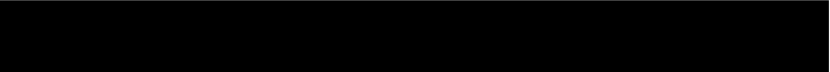
\includegraphics[width=1.2\paperwidth]{Logos/UCL page footer.png}
      }}
      

\thispagestyle{headings}
\maketitle
\FloatBarrier
\pagenumbering{roman}

\thispagestyle{empty}
\begin{abstract}
%\lipsum[5]
Testing absttact
%1.Talks about general application or general field of research
%2. Explains the challenge that is not answered yet
%3. Describe idea for tackling that challenge e.g. overall idea
%4 Methodology undertaken in research  e.g. tools, methods, steps taken.
%5. Main achievement of research supported by numerical results
%6. comparison with similar research in literature (qualitatively or quantitatively), and/or explain possible future applications of outcomes


\keywords{keyword 1 - keyword 2 - keyword 3}
% \vspace{-10mm} %To remove added white space after
\end{abstract}
\newpage
\thispagestyle{empty}
\begin{center}
I dedicate this ...
\end{center}

\newpage
\thispagestyle{empty}
\vspace*{\fill}
\begin{center}
Copyright \copyright  \thinspace 2023 by Andr\'{e}s Restrepo Jim\'{e}nez \\ All Rights Reserved
\end{center}
\vspace*{\fill}
\newpage
\thispagestyle{empty}
%\epigraph{The Book of Nature is written in the language of mathematics.}{--- \textup{Galileo Galilei}}
\epigraph{The computer was born to solve problems that did not exist before.}{--- \textup{Bill Gates}}


\thispagestyle{empty}
\chapter*{Acknowledgements}


\thispagestyle{empty}
\chapter*{Declaration}
I, Andr\'{e}s Restrepo Jim\'{e}nez, hereby declare that this dissertation is all my own original work and that all sources have been acknowledged. It is xxx words in length. \\
Add signature png here.
\begin{figure}[H]

\includegraphics{Logos/Signature.jpg}
\end{figure}
\vspace{-2cm}
\noindent\begin{tabular}{ll}
 & 20/08/23 \\
\makebox[2.5in]{\hrulefill} & \makebox[2.5in]{\hrulefill}\\
\textit{Signature} & \textit{Date}\\
\end{tabular}



\tableofcontents
\pagenumbering{arabic}
\thispagestyle{plain}
\listoffigures
\listoftables
%\lstlistoflistings
%\listofalgorithms


%\begin{singlespace}
\chapter*{List of acronyms or abbreviations}
\begin{sortedlist} %sort alphabetically
  \sortitem{BRT: Bus rapid transit}
  \sortitem{GIS: Geopraphic information system}
  \sortitem{GTFS: General transit feed specification}
  \end{sortedlist}
% \end{singlespace}
%%%%%%%%%%%%%%%%%%%%%%%%%%%%%%%%%%%%%%%%%%%%%%%%%%%%%%%%%%%%%%%%%%%%%%%%%%%%%%%%
%\input{1 Introduction}
%%%%%%%%%%%%%%%%%%%%%%%%%%%%%%%%%%%%%%%%%%%%%%%%%%%%%%%%%%%%%%%%%%%%%%%%%%%%%%%%
%\input{2 Literature review}
%%%%%%%%%%%%%%%%%%%%%%%%%%%%%%%%%%%%%%%%%%%%%%%%%%%%%%%%%%%%%%%%%%%%%%%%%%%%%%%%
%\input{3 Study area and or data chapter}
%%%%%%%%%%%%%%%%%%%%%%%%%%%%%%%%%%%%%%%%%%%%%%%%%%%%%%%%%%%%%%%%%%%%%%%%%%%%%%%%
%\input{4 Methodology}
%%%%%%%%%%%%%%%%%%%%%%%%%%%%%%%%%%%%%%%%%%%%%%%%%%%%%%%%%%%%%%%%%%%%%%%%%%%%%%%%
%\input{5 Results}
%%%%%%%%%%%%%%%%%%%%%%%%%%%%%%%%%%%%%%%%%%%%%%%%%%%%%%%%%%%%%%%%%%%%%%%%%%%%%%%%
%\input{6 Discussion}
%%%%%%%%%%%%%%%%%%%%%%%%%%%%%%%%%%%%%%%%%%%%%%%%%%%%%%%%%%%%%%%%%%%%%%%%%%%%%%%%
%\input{7 Conclusion}
%%%%%%%%%%%%%%%%%%%%%%%%%%%%%%%%%%%%%%%%%%%%%%%%%%%%%%%%%%%%%%%%%%%%%%%%%%%%%%%%
\chapter{Introduction} \label{Chap1}

\section{Background}

The first announcement of the construction of Bogota's future metro system was on XXXXXX by XXXX. On several occasions, the need for a higher-capacity public transportation system in Colombia's capital has taken great attention from the general public. The initial idea of building a metro in Bogot\'{a} goes back to the year 1942 when the current mayor at the time suggested the building of a new metro system as the functioning trolley car was highly demanded \citep{metrodebogotaHistoriaMetroBogota2011}. The previous versions of the project were unsuccessful in terms of their execution and compilation, however, each attempt reinforced the need of improving Bogota's public transportation system.

By September 2016, the local and national governments finally materialized their intentions in a formal agreement to support the development of the metro project which led to the ongoing construction process that started in 2021. The project consists of the construction of the first of two future metro lines. The scope of this research will only include the first metro line in the future scenario as the final designs of the second metro line have not been published yet. 

The first metro line will have a 23,9-kilometre length overground track with 16 stations. With an investment of 12,95 billion COP (4,33\footnote{September 2017 average COP/USD rate: 2.991,42 \citep{}} billion USD), the construction of the first line began in 2021 and is supposed to be finished and functional by 2028.



\begin{itemize}
 \item Lack of functioning metro system in Bogota although it has been proposed and mention in previous local and/or national government plans
    \begin{itemize}
      \item  For dimensions reference, mention bogotas demographics data.
    \end{itemize}
  \item How it contribute or prevent people to have better life quality
\end{itemize}

\section{Importance}

The importance of Colombia's capital, Bogot\'{a} can be measured from multiple angles. Population-wise, with XXX million people, the city accounts for X of the country's total population. Regarding the city's economic role, it is the biggest economic hub with X of the nation's GDP, followed by Medellín and Cali, with x and x, respectively.

\begin{itemize}

\item Brief intro to Bogota as a city and centre of economic and decision-making processes
\item It takes advantage of the use of publicly available data from transport and local authorities (spatial and non-spatial)
  \item Provide technical tools to assess transport planning decision
  \item Baseline reference for future or similar transport public policy decision making
  \item Assess how the metro system designs address the accessibility of the inhabitants
  \item Spatial reference for future local government intervention and investment decisions from the private sector
  \item Highlight accessibility importance in an economic and urban context and How can it drive growth
  \item Mention the impact on making cities more "liveable" and contribute to having a better life quality
\end{itemize}

\section{Research question}

The present research aims to address:

% Initial one


% \begin{center}
%     \textit{How would the public transportation accessibility spatially vary with the construction of Bogot\'{a}\textquotesingle s future metro system?}
% \end{center}

% Adjusted one

% \begin{center}
%     \textit{How would Bogot\'{a}\textquotesingle s future metro lines contribute to improving access to opportunities? To what extent is addressing the socio-spatial inequalities in Colombia\textquotesingle s capital?}
% \end{center}

% Current one

\begin{center}
    \textit{How would Bogot\'{a}\textquotesingle s future metro lines contribute to improving access to opportunities? How would the public transportation accessibility spatially vary with the construction of Bogot\'{a}\textquotesingle s future metro system?}
\end{center}



% \subsection{Subsection}
% \subsubsection{SubSubsection}
% \paragraph{Parragraph}
% \lipsum[5]
% Testing \Gls{raster}

Testing footnote\footnote{Capion of footnote!}

Testing references \citep{alcaldiamayordebogotad.c.EstacionesPrimeraLinea2022}
\chapter{Literature review} \label{Chap2}

\begin{itemize}
  \item Reference to Global UN Sustainability goals related to urban development and livable cities
  \item Reference to National (Colombia) and local government (Bogota) plans related to transport infrastructure (or in Chapter 3?)
  \item Reference to initiatives and efforts from NGO organizations related to urban accessibility: IBD, World Bank, GIZ.
  \item Modelling in the urban context
  \item Reference to north and global south previous research

  \item Reference to research done in Bogota (or in Chapter 3?)


\end{itemize}

\chapter{Study area and or data chapter} \label{Chap3}

\section{Bogot\'{a} summary (Should I do this in the introduction?)}

\begin{itemize}
  \item Brief context of Bogot\'{a} as Colombia\textquotesingle s capital
  \item Current Bogot\'{a}\textquotesingle s spatial structure
  \item Social and spatial population distribution
\end{itemize}

\section{Data}

\subsection{Population and demographics}

\subsection{Land use}

\subsection{Transport infrastructure}

\subsubsection{Bus Rapit Transit network}

\subsubsection{Metro network}



\chapter{Methodology} \label{Chap4}

\section{Accessibility measures}

\subsection{Cumulative accessibility}

\subsection{Minimum time to opportunities}

\section{Accessibility modelling}

\chapter{Results} \label{Chap5}
\chapter{Discussion} \label{Chap6}
\chapter{Conclusion} \label{Chap7}


\renewcommand{\bibname}{References}
\bibliographystyle{abbrvnat}
%\bibliography{Bibliography.bib}
\bibliography{references.bib}
%%%%%%%%%%%%%%%%%%%%%%%%%%%%%%%%%%%%%%%%%%%%%%%%%%%%%%%%%%%%%%%%%%%%%%%%%%%%%%%%
% APPENDIX
\begin{appendices}
\chapter{Source code and data} \label{System Requirements}
Source code and data for all of the methods implemented in Chap. \ref{Chap4} for the project can be found in the remote repository: \href{https://github.com/rpoandres/MSc_USS_Dissertation}{GitHub}



% \chapter{Project Introduction Video}\label{sec:projectIntroduction}
% A short video presentation, introducing background, aims and organisation of the project, as of 30$^{th}$ June 2022: \newline
% \url{link}



\end{appendices}
%%%%%%%%%%%%%%%%%%%%%%%%%%%%%%%%%%%%%%%%%%%%%%%%%%%%%%%%%%%%%%%%%%%%%%%%%%%%%%%%
% GLOSSARY
\clearpage
\printglossaries

% INDEX?

\end{document}